\documentclass[letterpaper,11pt]{article}

\usepackage{latexsym}
\usepackage[empty]{fullpage}
\usepackage{titlesec}
\usepackage{marvosym}
\usepackage[usenames,dvipsnames]{color}
\usepackage{verbatim}
\usepackage{enumitem}
\usepackage[hidelinks]{hyperref}
\usepackage{fancyhdr}
\usepackage[english]{babel}
\usepackage{tabularx}
\usepackage{fontawesome5}
\usepackage{multicol}
\setlength{\multicolsep}{-3.0pt}
\setlength{\columnsep}{-1pt}
\input{glyphtounicode}

%new packages

\usepackage{fontenc}
\usepackage{amsmath}
\usepackage{amssymb}
\usepackage{graphicx}



%----------FONT OPTIONS----------

\pagestyle{fancy}
\fancyhf{} % clear all header and footer fields
\fancyfoot{}
\renewcommand{\headrulewidth}{0pt}
\renewcommand{\footrulewidth}{0pt}

% Adjust margins
\addtolength{\oddsidemargin}{-0.6in}
\addtolength{\evensidemargin}{-0.5in}
\addtolength{\textwidth}{1.19in}
\addtolength{\topmargin}{-.7in}
\addtolength{\textheight}{1.4in}

\urlstyle{same}

\raggedbottom
\raggedright
\setlength{\tabcolsep}{0in}

% Sections formatting
\titleformat{\section}{
  \vspace{-4pt}\scshape\raggedright\large\bfseries
}{}{0em}{}[\color{black}\titlerule \vspace{-5pt}]



% Ensure that generate pdf is machine readable/ATS parsable
\pdfgentounicode=1

%-------------------------
% Custom commands
\newcommand{\resumeItem}[1]{
  \item\small{
    {#1 \vspace{-2pt}}
  }
}

\newcommand{\classesList}[4]{
    \item\small{
        {#1 #2 #3 #4 \vspace{-2pt}}
  }
}

\newcommand{\resumeSubheading}[4]{
  \vspace{-2pt}\item
    \begin{tabular*}{1.0\textwidth}[t]{l@{\extracolsep{\fill}}r}
      \textbf{#1} & \textbf{\small #2} \\
      \textit{\small#3} & \textit{\small #4} \\
    \end{tabular*}\vspace{-7pt}
}

\newcommand{\resumeSubSubheading}[2]{
    \item
    \begin{tabular*}{0.97\textwidth}{l@{\extracolsep{\fill}}r}
      \textit{\small#1} & \textit{\small #2} \\
    \end{tabular*}\vspace{-7pt}
}

\newcommand{\resumeProjectHeading}[2]{
    \item
    \begin{tabular*}{1.001\textwidth}{l@{\extracolsep{\fill}}r}
      \small#1 & \textbf{\small #2}\\
    \end{tabular*}\vspace{-7pt}
}


\newcommand{\resumeSubItem}[1]{\resumeItem{#1}\vspace{-4pt}}

\renewcommand\labelitemi{$\vcenter{\hbox{\tiny$\bullet$}}$}
\renewcommand\labelitemii{$\vcenter{\hbox{\tiny$\bullet$}}$}

\newcommand{\resumeSubHeadingListStart}{\begin{itemize}[leftmargin=0.0in, label={}]}
\newcommand{\resumeSubHeadingListEnd}{\end{itemize}}
\newcommand{\resumeItemListStart}{\begin{itemize}}
\newcommand{\resumeItemListEnd}{\end{itemize}\vspace{-5pt}}



\begin{document}
\fontfamily{cmr}\selectfont
\begin{center}
\parbox{3.0cm}{%
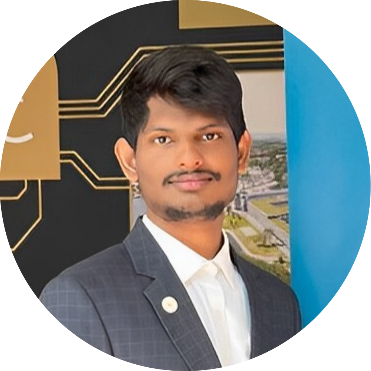
\includegraphics[width=2.7cm,clip]{images/resume_pic_m.png}}
}
\parbox{\dimexpr\linewidth-3.8cm\relax}{
\vspace{-20pt}
\begin{tabularx}{\linewidth}{L r} \\
    {\Huge \scshape  Venkata Sai Yakkshit Reddy Asodi}~
    \href{https://www.cedzlabs.com/yakkshit}{\vspace{1pt}}\\
      Berlin, Germany \\ \vspace{1pt}
     \small \raisebox{-0.1\height}\faPhone\ +91 9493006444 ~ \href{mailto:saiyakkshit2001@gmail.com}{\raisebox{-0.2\height}\faEnvelope\  {saiyakkshit2001@gmail.com}} ~ 
    \href{https://linkedin.com/in/yakkshit/}{\raisebox{-0.2\height}\faLinkedin\ {yakkshit}}  ~
    \href{https://yakkshit.com/}{\raisebox{-0.2\height}\faGlobe\ {yakkshit.com}}  ~
    \href{https://github.com/yakkshit}{\raisebox{-0.2\height}\faGithub{ yakkshit}}
    \vspace{-8pt}
\end{tabularx}
}
\end{center}

\vspace{-23pt}
\href{https://www.yakkshit.com/#details}{\section{Summary \faLink}
Experienced Backend Developer with strong expertise in PHP/Symfony framework and distributed systems architecture. Proven track record in developing scalable applications with focus on Test-Driven Development and continuous integration. Skilled in optimizing system performance and implementing robust caching solutions. Fluent in English (C1 level) with excellent communication abilities and a quality-driven approach to software development.}

\section{\href{https://www.linkedin.com/in/yakkshit/details/skills/}{Technical Skills} \faLink}
\begin{itemize}[leftmargin=0.15in, label={}]
\small{\item{
\textbf{Backend - }{PHP 8.x, Symfony 6.x, Object-Oriented Programming, REST APIs} \\
\textbf{Databases \& Caching - }{MySQL, Redis, ElasticSearch, Database Optimization} \\
\textbf{Testing \& CI/CD - }{PHPUnit, TDD, Jenkins, GitLab CI, Docker} \\
\textbf{Architecture - }{Microservices, Distributed Systems, Service-Oriented Architecture}\\
}}
\end{itemize}
\vspace{-10pt}

\section{Experience \faLinkedin}
\resumeSubHeadingListStart

\resumeSubheading
{\large Circleup AG \faBuilding}{December 2023 -- July 2024}
{Senior Backend Developer}{\faMapMarker \hspace{0.1cm} Zurich, Switzerland}\\
\vspace{10pt}
\textbf{Responsibilities:}
\resumeItemListStart
\vspace{-10pt}
\resumeItem{Architected and implemented scalable backend solutions using PHP/Symfony, improving system performance by 60\%}
\resumeItem{Established Test-Driven Development practices, achieving 90\% test coverage and reducing bug incidents by 75\%}
\resumeItem{Implemented Redis caching strategy that reduced database load by 40\% and improved response times by 65\%}
\resumeItemListEnd
\vspace{-3pt}
\textbf{Environment:}\emph{PHP, Symfony, MySQL, Redis, ElasticSearch, Docker}

\resumeSubheading
{Cedzlabs \faBuilding}{March 2023 -- November 2023}
{Backend Developer}{\faMapMarker \hspace{0.1cm} Berlin, Germany}\\
\vspace{10pt}
\textbf{Responsibilities:}
\vspace{-10pt}
\resumeItemListStart
\resumeItem{Developed and maintained RESTful APIs using Symfony framework, serving 100,000+ daily requests}
\resumeItem{Implemented automated CI/CD pipeline reducing deployment time by 70\% and increasing release reliability}
\resumeItemListEnd
\vspace{-3pt}
\textbf{Environment:}\emph{PHP, Symfony, MySQL, GitLab CI, PHPUnit}


\resumeItem{\textbf{\href{https://linkedin.com/in/yakkshit}{Checkout my other experiences by clicking here}}}
\vspace{-5pt}

\section{Projects \faGithub}
\vspace{-5pt}
\resumeSubHeadingListStart
\resumeProjectHeading
{\textbf{\href{https://ui.cedzlabs.com/resume}{E-Commerce Backend}} $|$ \emph{PHP/Symfony, MySQL, Redis}}{2024}\\
\vspace{6pt}
\textbf{Description:}
\vspace{-5pt}
\resumeItemListStart
\resumeItem{Developed a high-performance e-commerce backend using Symfony and MySQL. Implemented advanced caching with Redis, automated testing suite with PHPUnit, and continuous integration pipeline. The system handles 500+ transactions per minute with 99.9\% uptime.}
\resumeItemListEnd
\vspace{4pt}
\textbf{Tools:}\emph{
Symfony, MySQL, Redis, PHPUnit, Docker, GitLab CI}
\vspace{-10pt}

\resumeProjectHeading
{\href{https://yakkshit.com}{\textbf{Distributed Cache System}} $|$ \emph{PHP, Redis, ElasticSearch}}{2023}\\
\vspace{6pt}
\textbf{Description:}
\vspace{-5pt}
\resumeItemListStart
\resumeItem{Built a distributed caching system using Redis and ElasticSearch for high-traffic web applications. Implemented fault tolerance, automatic failover, and cache invalidation strategies. Reduced average response time from 300ms to 50ms.}
\resumeItemListEnd
\vspace{4pt}
\textbf{Tools:}\emph{PHP, Redis, ElasticSearch, Docker}
\vspace{-12pt}

\section{Achievements / Technical Expertise}
\resumeSubHeadingListStart
\resumeItemListStart
\resumeItem{Implemented microservices architecture that scales to handle 1M+ daily requests}
\resumeItem{Reduced deployment failures by 90\% through robust CI/CD implementation}
\resumeItem{Contributed to Symfony community with several accepted pull requests}
\resumeItemListEnd

\resumeSubHeadingListEnd
\textbf{Strengths:}\emph{System Architecture, Performance Optimization, Test-Driven Development, Team Collaboration} \\
\textbf{Education:}\emph{Bachelor of Technology in Computer Science, JNTU Hyderabad (2019-2023)} \\
\textbf{Languages:}\emph{English - C1 Level $|$ German - B1 Level $|$ Telugu - Native $|$ Hindi - Fluent}

\vspace{10pt}
\end{document}